% !TEX root = pfe-book1.tex
%!TEX TS-program = pdflatex
%!TEX encoding = UTF-8 Unicode


\cleardoublepage
\chapter{Laws of Motion}
\label{02-motion}

\section{Various Points of View About Motion}

The valise is standing in the baggage rack. At the same time, it is moving together with the train. The house is standing on the Earth, but it is also moving together with it. It is possible to say about one and the same body: it is moving in a straight line, it is at rest, it is rotating. And all these statements will be true, but from different points of view.

Not only the graph of the motion but also its properties can be
entirely different if regarded from different points of view.

Recall what happens to objects on a ship which is being rocked by the sea. How they misbehave! The ash-tray on the table overturned and dove headlong under the bed.  The water splashes in the bottle, and the lamp vibrates like a pendulum. Without any visible cause, some objects begin moving and others stop. An observer on such a ship might say that the basic law of motion is that at any moment an unfastened object can start travelling in any direction with an arbitrary speed.


This example shows that among the various points of view on motion
there are those which are really awkward.

But what point of view is the most ``reasonable''?

If suddenly, for no reason whatsoever, the lamp on the table were to
bend over, or the paper-weight were to jump, then at first you would
think that it was only your imagination, If these miracles were
repeated, you would urgently start looking for the cause which drove
these bodies out of the state of rest.

It is therefore perfectly natural to regard the point of view on
motion, according to which bodies at rest do not budge without the
action of a force, as a rational one.  Such a point of view seems
quite natural: a body is at rest -- hence, the sum of the forces
acting on it is equal to zero; it moved -- this happened under the
action of a force.  

This point of view presupposes the presence of an observer. However,
it is not the observer himself who is of interest to us, but his
location. Therefore, instead of ``point of view on motion'', we shall
say ``frame of reference in which the motion is regarded'', or simply
``frame of reference''.

For us, inhabitants of
the Earth, an important frame of reference is the Earth. However,
bodies moving on the Earth, say, a ship or a train, can also
frequently serve as frames of reference.  

Let us now return to the ``point of view'' on motion which we called
rational. This frame of reference has a name -- it is called
\emph{inertial}.

We shall see a bit later where this term comes from.  

Consequently, the properties of an inertial frame of reference are as
follows: bodies in a state of rest with respect to such a frame of
reference do not feel the action of forces. Therefore, not a single
motion in such a frame of reference is begun without the action of a
force. The simplicity and convenience of such a frame of reference are
obvious. It would pay to study motion in them.  

The fact that the frame of reference associated with the Earth does
not differ greatly from an inertial one is extremely important. We can
therefore begin our investigation of the basic regularities of motion
considering them from the point of view of the Earth. Nevertheless, we
must bear in mind that, strictly speaking, everything that will be
said in the next section deals with an inertial frame of reference.

\section{The Law of Inertia}
There can be no quarrel -- an inertial frame of reference
is convenient and has invaluable advantages.

But is such a frame of reference unique or do there,
perhaps, exist many inertial frames of reference? The
Ancient Greeks, for example, took the former point of
view. In their writings we find many na\"ive reflections
on the causes of motion. These ideas find their completion
in Aristotle. In the opinion of this philosopher, the
natural state of a body is rest -- of course, with respect
to the Earth. Every displacement of a body with respect
to the Earth must have a cause -- a force. But if there is
nothing causing a body to keep moving, it must halt,
return to its natural state. And this is what rest with
respect to the Earth is. From this point of view, the
Earth is the unique inertial frame of reference.

We are indebted to the great Italian Galileo Galilei
(1564-1642) for discovering the truth and disproving
this false but congenial to naive psychology opinion.

Let us think over the Aristotelian explanation of
motion and search familiar phenomena for confirmation
or refutation of the idea that rest is the natural state
of bodies on the Earth.

Imagine that we are in an airplane taking off from an
airport at dawn. The Sun has not yet warmed up the air,
so there are no ``air-pockets'', which cause many passengers unpleasantness. The airplane is moving smoothly,
imperceptibly. If you don't look out of the window, you
won't even notice that you're flying. A book is lying on
an empty seat; an apple is at rest on a table. All objects
inside the airplane are motionless. Is this how things
should be if Aristotle were right? Of course not. As a
matter of fact, according to Aristotle, the natural state
of a body is rest on the Earth. But then why are all the
objects not piled up at the rear wall of the airplane
trying to lag behind its motion, ``wanting'' to return to
the state of ``true'' rest? What makes the apple lying on
the table, hardly touching the surface of the table, move
with an enormous speed of several hundred kilometres
an hour?

What is the correct answer to the question of the
cause of motion? Let us first take up the question of why
moving bodies come to a stop. For example, why does
a ball rolling along the Earth's surface come to a stop?
In order to give a correct answer, we should consider
in which cases a ball comes to a stop quickly, and in
which cases slowly. We don't need any special experiments for this. We know perfectly well from our practical
experience that the smoother the surface on which a ball
is moving, the farther it will roll. From these and similar
experiences, there arises the natural idea of the force
of friction as a hindrance to motion, as the cause for the
slowing down of an object which is rolling or slipping'
along the Earth. Friction can be decreased in various
ways. The more we work on the destruction of every
kind of resistance to motion (for example, the smoother
we construct our roads, the better we lubricate our engines
and the more we perfect our ball bearings), the greater
the distance a moving body will cover freely without
being acted on by any external force.

The following question arises: What would happen if
there were no resistance, if the force of friction were
absent? Obviously, in such a case a motion would continue
infinitely, with a constant speed and along one and the
same straight line.
%\newpage

\begin{center}
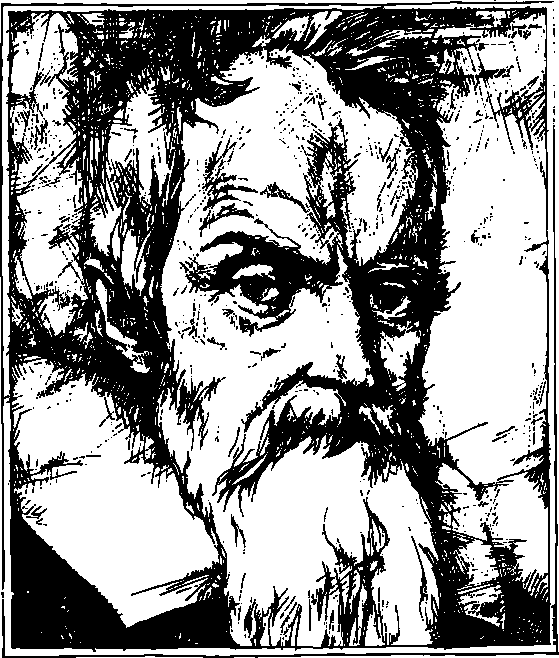
\includegraphics[width=0.8\textwidth]{figures/galileo.pdf}
\end{center}
{\small \textsf{{Galileo Galilei [1564-1641]}} -- \textsf{\footnotesize a great Italian physicist and astronomer, the first to apply the experimental method of investigation
in science. Galileo introduced the concept of inertia, established
the relativity of motion, investigated the laws of free fall, of the motion of bodies on an inclined plane, and of the motion of an
object thrown at an angle to the horizontal, used a pendulum for
the measurement of time. For the first time in the history of
mankind, he looked at the sky through a telescope, discovered
many new stars, proved that the Milky Way consists of an enormous number of stars, discovered Jupiter's satellites, sunspots and
the rotation of the Sun, investigated the structure of the Moon's
surface. Galileo actively supported Copernicus' heliocentric system banned in those days by the Catholic church. Persecution by the Inquisition darkened the last ten years of the great scientist's
life.}}



We have formulated the law of inertia in about the
same form as it was first given by Galileo. Inertia is
a brief designation for this ability of a body to move rectilinearly and uniformly without any cause, contrary to Aristotle. Inertia is an inalienable property of each particle in the Universe.

In what way can we check the validity of this remarkable law? As a matter of fact, it is impossible to create
conditions under which no forces would be acting on a
moving body. Even though this is true, we can, on the
other hand, observe the opposite. In every case when
a body changes the speed or direction of its motion, it
is always possible to find a cause -- a force responsible
for this change.

A body acquires speed in falling to the Earth; the cause
is the Earth's gravitation. A stone twirls on a string
circumscribing a circle; the cause deflecting the stone
from a rectilinear path is the tension in the string. If
the string breaks, the stone will fly off in the same direction in which it was moving at the moment the string
broke. An automobile running with the motor turned off
slows down; the causes are air resistance, friction between
the tires and the road, and imperfections in the ball
bearings.

The law of inertia is the foundation on which the
entire study of the motion of bodies rests.


\section{Motion Is Relative}

The law of inertia leads to the derivation of the multiplicity of inertial frames of reference. Not one but many frames of reference exclude ``causeless'' motions.

If one such frame of reference is found, we can immediately find another, moving (without rotation) uniformly and rectilinearly with respect to the first. Moreover, one inertial frame of reference is not the least bit better than the others, does not in any way differ from the others. It is in no way possible to find a best frame of reference among the multitude of inertial frames of reference. The laws of motion of bodies are identical in all inertial frames of reference: a body is brought into motion only under the action of forces, is slowed down by forces, and in the absence of any forces acting on it either remains at rest or moves uniformly and rectilinearly.

The impossibility of distinguishing some particular inertial frame of reference with respect to the others by means of any experiments whatsoever constitutes the essence of the \emph{Galilean principle of relativity} -- one of the most important laws of physics.

But even though the points of view of observers studying phenomena in two inertial frames of reference are fully equivalent, their judgements about one and the same fact will differ. For example, one of the observers will say that the seat on which he is sitting in a moving train is located at the same place in space all the time, but another observer standing on the platform will assert that this seat is moving from one place to another. Or one observer firing a rifle will say that the bullet flew out with a speed of \SI{500}{\meter\per\second}, while another observer, if he is in a frame of reference which is moving in the same direction with a speed of \SI{200}{\meter\per\second}, will say that the bullet is flying considerably slower, with a speed of \SI{300}{\meter\per\second}. 

Who of the two is right? Both. For the principle of the
relativity of motion does not allow a preference to be
given to any single inertial frame of reference.

It turns out that no unconditionally true (as is said,
absolute) statements can be made about a region of space
or the velocity of motion. The concepts of a region of
space and the velocity of motion are relative. In speaking
about such relative concepts, it is necessary to indicate
which inertial frame of reference one has in mind.

Therefore, the absence of a single unique ``correct'' point
of view on motion leads us to recognize the relativity of
space. Space could have been called absolute only if we
were able to find a body at rest in it-at rest from the
point of view of all observers. But this is precisely what
is impossible to do.

The relativity of space means that space may not be
pictured as something into which bodies have been immersed.

The relativity of space was not recognized immediately
by science. Even such a brilliant scientist as Newton
regarded space as absolute, although he also understood
that it would be impossible to prove this. This false point
of view was widespread among a considerable number of
physicists up to the end of the $19^{\textrm{th}}$ century. The reasons for this are apparently of a psychological nature: we are
simply very much accustomed to see the immovable
``same places in space'' around us.

We must now figure out what absolute judgements can he made about the character of motion.

If bodies move with respect to one frame of reference
with velocities $\mathbf{v_{1}}$ and $\mathbf{v_{2}}$ then their difference (vector, of course) $\mathbf{v_{1}} - \mathbf{v_{2}}$ will be identical for any inertial observer, since both of the velocities $\mathbf{v_{1}}$ and $\mathbf{v_{2}}$ undergo the same change when the frame of reference is changed.

Thus, the vector difference between the velocities of two bodies is absolute. If so, the vector increment in the velocity of one and the same body for a definite interval of time is also absolute, i.e. its value is identical for all inertial observers.

\section{The Point of View of a Celestial Observer}

We decided to study motion from the point of view of an inertial frame of reference. Won't we then have to reject the services of the terrestrial observer? As a matter of fact, the Earth rotates about its axis and revolves around the Sun, as was proved by Nicolaus Copernicus (1473-1543). It may be difficult for the reader to feel now how revolutionary Copernicus' discovery was to realize that Giordano Bruno was burned at the stake, and Galileo suffered humiliation and exile for championing the truth of Copernicus' ideas.

What was it that Copernicus' genius accomplished? Why may we place the discovery of the Earth's rotation and revolution on one plane with the ideas of human justice for which progressive-minded people have been willing to give up their lives?

In his \emph{Dialogue on the Two Chief Systems of the World} (the Ptolemaic and the Copernican), for whose writing he was persecuted by the Inquisition, Galileo gave the opponent of the Copernican system the name Simplicio, which means ``simpleton''.

In fact, from the point of view of a simple direct observer of the world, that which is not very aptly called ``common sense'', the Copernican system seems mad. How can the Earth rotate? As a matter of fact, I see it and it is stationary, but the Sun and the stars are really moving.

The attitude of theologians to Copernicus' discovery is shown by the following conclusion of the Assembly of Theologians (1616): \begin{quote}
The doctrine that the Sun is located at the centre of the world and is immovable is false and absurd, formally heretical and contrary to the Bible. More than that, the doctrine that the Earth does not lie at the centre of the world and moves, possessing in addition a daily rotation, is false and absurd from the philosophical point of view and at least erroneous from the theological one.
\end{quote}

This conclusion, in which a lack of understanding of the
laws of nature and a belief in the infallibility of religious
dogmas are mixed up with a false ``common sense'', testifies better than anything else to the strength of Copernicus' spirit and mind, and those of his disciples having so resolutely broken with the ``truths'' of the $17^{\textrm{th}}$ century.

But let us return to the question posed above.

If the velocity of an observer's motion changes or if
he rotates, he must be deleted from the list of ``correct''
observers. But it is precisely under these conditions that
an observer on the Earth is found. However, if the change
in velocity or the observer's rotation during the time
he is investigating a motion is small, such an observer
may be conditionally regarded as ``correct''. Will this
pertain to an observer on the Earth?

During a second the Earth will turn 1/240 of a degree,
i.e. about \num{0.00007} radian. This isn't very much. The
Earth is therefore quite inertial with respect to a great
many phenomena.

Nevertheless, one can no longer forget about the Earth's rotation when dealing with prolonged phenomena. 

Under the dome of St. Isaac Cathedral in Leningrad hangs an enormous pendulum. If we start oscillating this pendulum, within a short time it will be possible to notice that the plane of its oscillation is slowly turning. After several hours, the plane of oscillation will turn through, a noticeable angle. Such an experiment with this kind of pendulum was first performed by the French scientist Leon Foucault (1819-1868), and has born his name ever since. The Foucault experiment yields a visual demonstration of the Earth's rotation (\figr{fig-2.01}).
\begin{figure}[!ht]
\centering
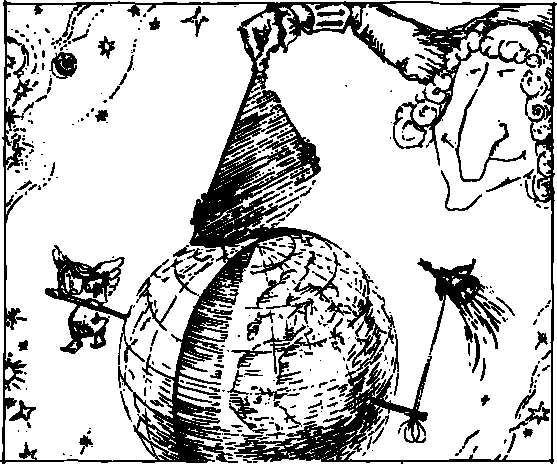
\includegraphics[width=\textwidth]{figures/fig-02-01.pdf}
\caption{The Foucault's pendulum.}
\label{fig-2.01}
\end{figure}

Thus, if the observed motion continues for a long time, we shall be forced to reject the services of the terrestrial observer and take a frame of reference associated with the Sun and the stars as our ba sis. Such a frame of reference was used by Copernicus assuming the Sun and the surrounding stars to be fixed. However, in reality Copernicus' frame of reference is not completely inertial.

The Universe consists of a great number of star-clusters -- islands of the Universe, which are called galaxies. In the galaxy to which our solar system belongs, there, are approximately one-hundred billion stars. The Sun is revolving around the centre of this galaxy with a period of about 180 million years and a speed of \SI{250}{\kilo\meter\per\second}. What error will be made by assuming a solar observer to be inertial?

For a comparison of the merits of terrestrial and solar
observers, let us compute the angle through which the
solar frame of reference turns during a second. If a complete revolution takes place every \num{180d6} years
$(\SI{6d15}{\second})$, then in one second the solar frame of reference will turn through an angle of \num{6d-14} degree or \num{d-15} radian. We may say that the solar observer is 100 billion times ``better'' than the terrestrial one.

Desiring an even closer approximation to an inertial
frame of reference, astronomers take a frame of reference
associated with several galaxies as a basis. Such a frame
of reference is the most inertial of all possible kinds. It
is impossible to find a better frame of reference.

Astronomers may be called star gazers in two senses:
they observe stars and describe the motions of heavenly
bodies from the point of view of the stars.

\section{Acceleration and Force}

In order to characterize the velocities that are not constant, physicists use the concept of acceleration. 

The change in velocity during a unit of time is called \emph{acceleration}. Instead of saying ``the velocity of a body changed by a in 1 second'', we say more briefly ``the acceleration of a body is equal to $a$.''

If we denote by $v_{1}$ the speed of a rectilinear motion at
the first instant, and by $v_{2}$ at the next, the rule for calculating the acceleration $a$ is expressed by the formula
\begin{equation*}
a = \frac{v_{2} - v_{1}}{t}
\end{equation*}
where $t$ is the time during which the speed builds up.

Speed is measured in \si{\centi\meter\per\second} (or \si{\meter\per\second}, etc.), time in seconds. Hence, acceleration is measured in \si{\centi\meter\per\second} per second. A number of centimetres per second is divided by seconds. Thus, the unit of acceleration will be \si{\centi\meter\per\second\squared}
(or \si{\meter\per\second\squared}, etc.).

Of course, the acceleration can change during the course
of a motion. However, we shall not complicate our treatment with this inessential fact. We shall implicitly assume that the velocity changes uniformly during the course of a motion. Such a motion is called \emph{uniformly accelerated}.

What is acceleration of curvilinear motion? 

Since velocity is a vector, a change (difference) in velocity is a vector, and so acceleration is also a vector. In order to find the acceleration vector, one must divide the vector difference between the velocities by the time. But we have already described how to construct a vector change in velocity.

The highway takes a turn. Let us note two nearby
positions of a car and represent its velocities by vectors
(\figr{fig-2.02}). Subtracting these vectors, we obtain a
quantity which is by no means equal to zero; dividing
it by the elapsed time, we find the acceleration vector.
An acceleration took place even when the speed around
the turn did not change. Curvilinear motion is always
accelerated. Only uniform rectilinear motion is unaccelerated.
\begin{figure}[!ht]
\centering
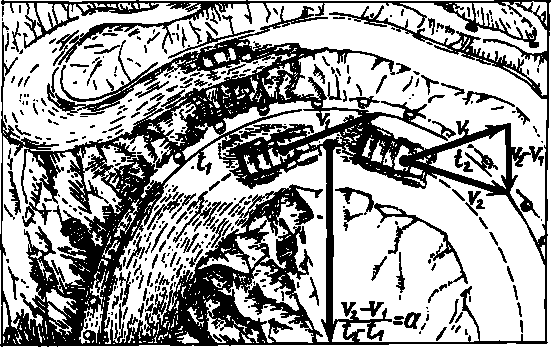
\includegraphics[width=\textwidth]{figures/fig-02-02.pdf}
\caption{Analysing motion of a car turning on a highway.}
\label{fig-2.02}
\end{figure}

In speaking about the velocity of motion of a body,
we always stipulated what our point of view was with
regard to the motion. The velocity of a body is relative.
From the point of view of one inertial frame of reference
it can be great, and from the point of view of another
inertial frame of reference it can be small. Don't we have
to make the same kind of stipulations when speaking
about acceleration? Of course not. Unlike velocity, acceleration is absolute. From the point of view of all imaginable inertial frames of reference acceleration will be identical. As a matter of fact, acceleration depends on the difference in the velocity of a body between the first and second instants of time, and this difference, as we already know, will be identical from all points of view,
i.e. is absolute.

If no force is acting on a body, it can only move without acceleration. Conversely, the action of a force on a body accelerates it; moreover, the greater the force, the greater will be the acceleration. The faster we want to move a loaded waggon, the more we have to strain our muscles. As a rule, two forces act on a moving body: accelerating -- the pull, and decelerating -- the force of friction or air resistance.

The difference between these two forces, the so-called
resultant force, may be directed along or against the
motion. In the first case, the body speeds up its motion;
in the second case, it slows it down. If these oppositely
acting forces are equal to each other, the body will move
uniformly, just as though there were no forces acting
on it.

But how is a force related to the acceleration it creates?
The answer turns out to be very simple. The acceleration
is proportional to the force:
\begin{equation*}%
F \propto a
\end{equation*}
(The symbol $\propto$ denotes ``is proportional to''.)

Another question still remains to be answered: How do
the properties of a body influence its ability to accelerate
its motion under the action of one or another force? For
it is clear that one and the same force acting on different
bodies will give them different accelerations.

We shall find the answer to the question we have posed
in the remarkable fact that all bodies fall to the Earth
with the same acceleration. This acceleration is denoted
by the letter $g$. In the vicinity of Moscow $g = \SI{981}{\centi\meter\per\second\squared}$.

Direct observation will not, at first sight, confirm the
identity of acceleration for all bodies. The fact is that
when a body is falling under ordinary conditions, besides
gravity there is another, ``hindering'' force acting on it --
air resistance. Philosophers of antiquity were quite confused by the difference in the way light and heavy bodies fall. A piece of iron falls quickly, but a feather glides through the air. A sheet of paper falls slowly to the ground, but if we roll it up, this same sheet will fall considerably faster. The fact that the atmosphere distorts
the ``true'' picture of the motion of a body under the action of the Earth was already understood by the Ancient Greeks. However, Democritus thought that even if the air were deleted, heavy bodies would always fall faster than light ones. But air resistance can have the opposite
effect, for example, a sheet of aluminium foil (all unrolled) will fall more slowly than a small ball made by crumpling a piece of paper.

Incidentally, metallic wire of such a thinness (several
microns) is so manufactured now that it glides through
the air like a feather.

Aristotle thought that all bodies should fall identically
in a vacuum. However, he used this theoretical conclusion
to make the following paradoxical deduction: ``The falling
of different bodies with the same speed is so absurd that
the impossibility of the existence of vacuum is
clear.''

None of the scientists of antiquity or the Middle Ages
guessed that it could be experimentally verified whether
bodies fall to the Earth with different or the same accelerations. Only Galileo demonstrated by means of his remarkable experiments (he investigated the motion of balls down an inclined plane and the fall of bodies thrown from the top of the leaning tower of Pisa\footnote{We have it on good authority that Galileo never performed the experiments involving dropping bodies from the leaning tower of Pisa. -- Damitr}) that
at any given point on the Earth all bodies fall with the
same acceleration, regardless of their mass. At the present time such experiments are quite easily performed with the aid of a long tube out of which the air has been pumped. A feather and a stone fall identically in such a tube: only one force acts on the bodies, and that is weight; air resistance has been reduced to zero. In the absence of air resistance, the fall of any body is a uniformly accelerated motion.

Let us now return to the question posed above. How
does the ability of a body to accelerate its motion under
the action of a given force depend on its properties?

Galileo's law states that all bodies, regardless of their
masses, fall with one and the same acceleration; hence,
a mass of $m \, \si{\kilo\gram}$ under the action of a force of $F \,\si{\kgf}$ moves with an acceleration $g$.

Now suppose we are no longer talking about falling bodies, and a force of \SI{1}{\newton} is acting on a mass of $m$ \si{\kilo\gram}. Since acceleration is proportional to force, it will be $m$
times less than $g$.

We have arrived at the conclusion that the acceleration
a of a body for a given force (\SI{1}{\kgf} in our example) is
inversely proportional to its mass.

Uniting both conclusions, we may write:
\begin{equation*}%
a \propto \frac{F}{m}
\end{equation*}
i.e, for a constant mass the acceleration is directly proportional to the force, and for a constant force inversely proportional to the mass.

This law, relating acceleration to the mass of a body
and the force acting on it, was discovered by the great
English scientist Sir Isaac Newton (1643-1727), and
bears his name.\footnote{Newton himself showed that motion is subject to three laws. The law which we are now discussing appears on Newton's
list as the seoond. He called the law of inertia the first law and the law of action and reaction the third.}

Acceleration is directly proportional to the acting
force and inversely proportional to the mass of a body,
and does not depend on any other properties of the body.
It follows from Newton's law that it is precisely the mass
which is the measure of the ``inertness'' of a body. For
identical forces, it is more difficult to accelerate a body
of greater mass. We see that the concept of mass, which
we first knew as a ``modest'' quantity determined by
weighing a body on a balance scale, has acquired a new
deep meaning: the mass characterizes the dynamic properties of a body.

Newton's law may be written as follows:
\begin{equation*}%
kF = ma
\end{equation*}
where $k$ is a constant coefficient. This coefficient depends
on the chosen units.


Instead of making use of the unit of force (\si{kgf}) we
already have available, we shall act in a different manner.
Just as physicists often try to do, we shall choose our
unit. Of force in such a way that the coefficient of proportionality in Newton's law becomes equal to unity. Then Newton's law takes the following form:
\begin{equation*}%
F = ma
\end{equation*}
As we have already said, in physics it is customary to
measure mass in grams, distance in centimetres, and time
in seconds. The system of units based on these three fundamental quantities is called the cgs system.

Let us now choose, using the principle formulated
above. the unit of force. A force will then obviously be
equal to unity when it imparts the acceleration of \SI{1}{\centi\meter\per\second\squared} to the mass of \SI{1}{\gram}. Such a force received the name \emph{dyne} in this system.

According to Newton's law, $F = ma$, the force will
be expressed in dynes if we multiply $m \, \si{\gram}$ by $a \, \si{\centi\meter\per\second\squared}$. One
therefore makes use of the following notation:
\begin{equation*}%
\SI{1}{\dyne} = \SI{1}{\gram\centi\meter\per\second\squared}
\end{equation*}
The weight of a body is usually denoted by the letter
$P$. The force $P$ gives the body an acceleration $g$, and in
dynes we obviously have
\begin{equation*}%
P = mg
\end{equation*}
But we already had a unit of force -- the kilogram-force
(\si{\newton}). We immediately find the relation between our
new and old units from the last formula:
\begin{equation*}%
\SI{1}{\newton} = \num{981 000} \, \textrm{dyn}
\end{equation*}
A dyne is a very small force. It is equal to about one
milligram of weight.

We have already mentioned the system of units (SI).
The name for the new unit of force, \emph{newton} (N), is fully
deserved. For such a choice of units, Newton's law will
look as simple as possible; this new unit is defined as
follows:
\begin{equation*}%
\SI{1}{\newton} = \SI{1}{\kilo\gram\meter\per\second\squared}
\end{equation*}
i.e. \SI{1}{\newton} is the force necessary to impart the acceleration
of \SI{1}{\meter\per\second\squared} to the mass of \SI{1}{\kilo\gram}.

It is not difficult to relate this new unit to the dyne and the kilogram-force:
\begin{equation*}%
\SI{1}{\newton} = \num{100000}\, \textrm{dyn} = \SI{0.102}{\kgf}
\end{equation*}


%\newpage

\begin{center}
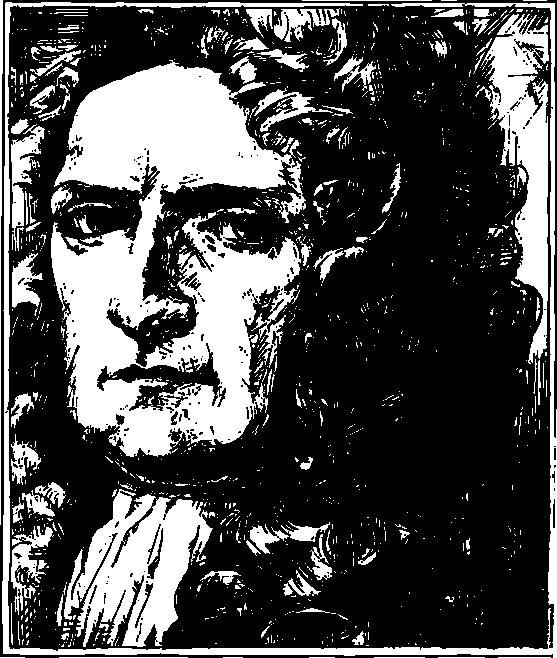
\includegraphics[width=0.8\textwidth]{figures/newton.pdf}
\end{center}

{\small \textsf{{Sir Isaac Newton [1643-1717]}} -- \textsf{\footnotesize a brilliant English physicist and
mathematician, one of the greatest scientists in the history of
mankind. Newton formulated the basic concepts and laws of
mechanics, discovered the law of universal gravitation, creating
by the same token a physical picture of the world with remained inviolable until the beginning of the 20th century. He
developed a theory of the motion of celestial bodies, explained
the most important special features of the Moon's motion and
gave an explanation for the tides. In optics, some remarkable
discoveries facilitating the rapid growth of this branch of physics are due to Newton. Newton devised a powerful method of the
mathematical investigation of nature; the honour of creating the
differential and integral calculus belongs to him. This exerted an
enormous influence on the entire subsequent development of
physics and facilitated the introduction of mathematical methods
of research.}}



\section{Rectilinear Motion with Constant Acceleration}

Such motion arises, according to Newton's law, when
the resultant force acting on a body, speeding it up or
slowing it down, is constant.

Such conditions arise rather frequently, even though
only approximately: a car moving with its motor cut off
slows down under the action of the more or less constant
force of friction: a weighty object falls from a height
under the action of the constant force of gravity.

Knowing the magnitude of the resultant force, and
also the mass of a body, we can find the magnitude of the
acceleration according to the formula $a = F/m$. Since
\begin{equation*}
a= \frac{v - v_{0}}{t}
\end{equation*}
where $t$ is the time of the motion, $v$ is the final speed, and
is the initial speed, with the aid of this formula it is
possible to answer a series of questions of, say, the following type: How long will it take a train to come to a halt if the decelerating force, the mass of the train and the initial speed are known? Or how much speed will a car gather if the power of the motor, the resistance, the mass of the car and the duration of acceleration are known?

We are often interested in knowing the distance covered by a body in a uniformly accelerated motion. If the motion is uniform, the distance covered is found by multiplying the speed of the motion by its time. If the motion is uniformly accelerated, the calculation of the distance covered is carried out as though the body were moving uniformly for the same time $t$ with the speed equal to half the sum of the initial and final speeds:
\begin{equation*}
s = \frac{1}{2} (v + v_{0}) \, t
\end{equation*}
Thus, for uniformly accelerated (or decelerated) motion,
the distance covered by a body is equal to the product
of half the sum of the initial and final speeds by the time
of the motion. The same distance would be covered during
the same time in a uniform motion with speed $(v_{0}+v)/2$. In this sense, one can say that $(v_{0}+v)/2$ is the average speed of the uniformly accelerated motion.

It is helpful to compose a formula which would show the dependence of the distance covered on the acceleration. Substituting $v = v_{0}
+ at$ in the last formula, we find:
\begin{equation*}
s = v_{0}t + \frac{1}{2} a t^{2}
\end{equation*}
or, if the motion occurs without any initial speed,
\begin{equation*}
s = \frac{1}{2} a t^{2}
\end{equation*}
If a body travels \SI{5}{\meter} in one second, then in two seconds it will travel $(4 \times 5) \, \si{\meter}$, in three seconds $(9 \times 5) \, \si{\meter}$, etc. The distance travelled grows in proportion to the
square of the time.

A heavy body falls from a height in accordance with this law. The acceleration of free fall is equal to $g$, and
our formula acquires the following form:
\begin{equation*}
s = \frac{981}{2} t^{2}
\end{equation*}
if $t$ is expressed in seconds and $g$ in centimetres per second per second.

If a body could fall without hindrance for some \SI{100}{\second},
it would cover an enormous distance from the beginning
of its fall -- about \SI{50}{\kilo\meter}. Moreover, only a mere \SI{0.5}{\kilo\meter} would be covered in the first \SI{10}{\second} -- this is what accelerated motion means.

But what speed will a body develop in falling from a
given height? To answer this question we shall need formulas relating the covered distance to the acceleration and the speed. Substituting the time of the motion $t = (v - v_{0})/a$ in $s = (1/2)(v_{0}+v) t$, we obtain:
\begin{equation*}
s = \frac{1}{2a}(v^{2} - v_{0}^{2})
\label{dist-time-acc}
\end{equation*}
or, if the initial speed is equal to zero,
\begin{equation*}
s = \frac{v^{2}}{2a} \quad v =\sqrt{2as}
\end{equation*}
Ten metres is the height of a small two- or three-storey
house. Why is it dangerous to jump to the ground from
the roof of such a house? A simple calculation shows that
the speed of such a free fall would reach the value $v =
\sqrt{2 \times 9.8 \times 10} \, \si{\meter\per\second} = \SI{14}{\meter\per\second} \approx \SI{50}{\kilo\meter\per\hour}$, and this
is, after all, the speed of a car within city limits.
Air resistance will not reduce this speed much.

The formulas we have singled out are employed for
the most varied computations. Let us apply them in order
to see how motions take place on the Moon.

In H. G. Wells' novel \emph{The First Men in the Moon} we read
about the surprises experienced by travellers in their
fantastic trips. On the Moon, the acceleration of gravity
is approximately six times less than terrestrial. If a falling body on the Earth covers \SI{5}{\meter} in the first second, it
will ``float'' down only \SI{80}{\centi\meter} in all on the Moon (the acceleration there is about \SI{1.6}{\meter\per\second}).

The formulas we have written out permit us to rapidly
calculate the lunar ``miracles''.

A jump from a height of $h \,\si{\meter}$ takes $t = \sqrt{2h/g} s$. Since lunar acceleration is six times less than terrestrial, the jump will require $\sqrt{6} \approx 2.45$ times more time on the Moon. By how many times will the final speed of the jump be: decreased $(v = \sqrt{2gh})$?

One can jump safely from the roof of a three-storey
house on the Moon. The height of a jump with the same
initial speed will be increased by a factor of six $(h = v^{2}/2g)$.
A child will be able to jump higher than the record set
on the Earth.

\section{Path of a Bullet}

People have been solving the problem of throwing an
object as far as possible from time immemorial. A stone
thrown by hand or shot from a sling, an arrow flown from a bow, a rifle bullet, an artillery shell, a ballistic missile -- here is a brief list of successes in this field.

The thrown object will move in a curved line called
a parabola. It can be constructed without difficulty if
we regard the motion of a thrown body as the sum of two
motions -- horizontal and vertical -- taking place simultaneously and independently. The acceleration of free fall
is vertical, and so a flying bullet moves horizontally by
inertia with a constant velocity and simultaneously falls
to the Earth vertically with a constant acceleration. But
how can we add these two motions?
\begin{figure}[!ht]
\centering
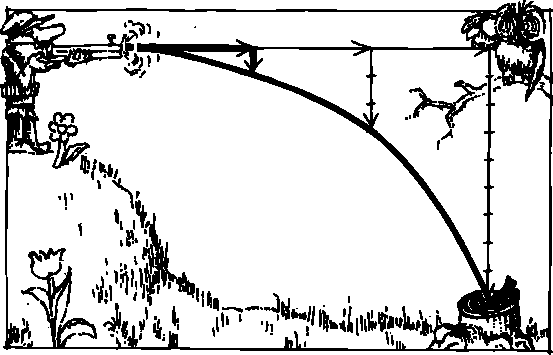
\includegraphics[width=\textwidth]{figures/fig-02-03.pdf}
\caption{Analysing motion of a shot from a rifle.}
\label{fig-2.03}
\end{figure}

Let us begin with a simple case -- when the initial
velocity is horizontal (say, we are dealing with a shot
from a rifle whose barrel is horizontal). Take a sheet of graph paper and draw a vertical and a horizontal lines (\figr{fig-2.03}). Since the two motions are taking place independently, in $t$ seconds the body is displaced by an interval of $v_{0}t$ to the right and an interval
of $gt^{2} /2$ downwards. Mark off the segment $v_{0}t$ along the
horizontal line, and from its end point, the vertical segment $gt^{2} /2$. The end point of the vertical segment represents the point where the body will be in $t$ seconds. This construction must be carried out for several points, i.e. for several instants of time. A smooth curve -- the parabola representing the trajectory of the body -- will pass through these points. The more frequently one lays off these points, the more accurately will the trajectory of the flight of the bullet be constructed.

A trajectory has been constructed in \figr{fig-2.04} for the
case when the initial velocity $v_{0}$ is directed at an angle.
The vector $v_{0}$ should first of all be decomposed into its
vertical and horizontal components. On the horizontal
line we mark off $v_{\textrm{hor}} t$ -- the distance through which the
bullet will move horizontally in $t$ seconds.
\begin{figure}[!ht]
\centering
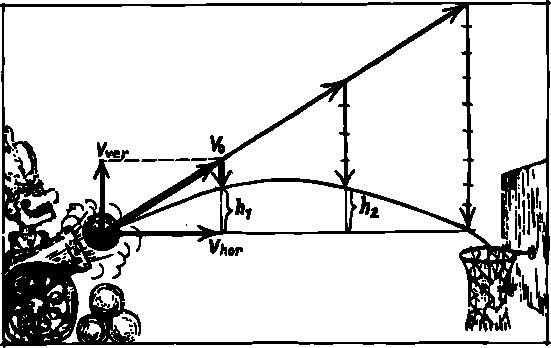
\includegraphics[width=\textwidth]{figures/fig-02-04.pdf}
\caption{Analysing a projectile trajectory.}
\label{fig-2.04}
\end{figure}
But the bullet simultaneously performs an upward
motion. In $t$ seconds it will rise to a height of $h =
 v_{\textrm{ver}} t - gt^{2} /2$. By means of this formula, substituting
in it the instants of time of interest to us, we can compute
the vertical displacements and mark them off on the
vertical axis. The values of $h$ will first increase (rise)
and then decrease.

It now remains to mark the points of the trajectory on
the graph, just as we did in the preceding example, and
draw a smooth curve through them.

If the rifle barrel is held horizontally, the bullet will
soon burrow into the ground; if the barrel is vertical, it
will fall at the place where the shot was fired. Therefore,
in order to shoot as far as possible, one must fix the barrel
of the rifle at some angle to the horizontal. But at what
angle?

Let us again employ the same device -- decompose the
initial velocity vector into its two components: a vertical
vector equal to $v_{1}$ and a horizontal vector to $v_{2}$. The
time between the moment the shot is fired until the moment
the bullet reaches its highest point is equal to $v_{1}/ g$. Note
that the bullet will be falling downwards for the same
length of time, i.e. the complete time of the flight of the
bullet until it lands on the ground is $2v_{1}/g$.

Since the horizontal motion is uniform, the range of the flight is equal to 
\begin{equation*}
s = \frac{2v_{1}v_{2}}{g} 
\end{equation*}
(we have ignored the height of the rifle above ground level
in our calculation).

We have obtained a formula which shows that the range
of the flight is proportional to the product of the velocity
components. For what firing direction will this product
be greatest? This question can be expressed by means of
the geometrical rule of the addition of vectors. The velocities $v_{1}$ and $v_{2}$ form the sides of the velocity rectangle; a diagonal in it is the total velocity $v$. The product $v_{1}v_{2}$ is equal to the area of this rectangle.

Our question reduces to the following: Given the length
of a diagonal, what sides must be taken for the area of
the rectangle to be maximum? It is proved in geometry
that this condition is satisfied by a square. Therefore, the
range of the flight of the bullet will be greatest when
$v_{1} = v_{2}$ , i.e. when the velocity rectangle reduces to a
square. A diagonal of the velocity square forms an angle
of \ang{45} with the horizontal -- this is precisely the angle
at which the rifle must be held for the bullet to fly as far
as possible.

If $v$ is the total velocity of the bullet, then in the case 2. The range-of-flight of a square we have $v_{1} = v_{2} =v\sqrt{2}$
formula for this optimal case looks as follows: $s = v^{2}/g$,
i.e. the range will be twice as great as the maximum height
of a bullet fired upwards with the same initial speed.

The maximum height of a bullet fired at an angle of \ang{45} will be $h = v_{1}^{2}/2g = v^{2}/4g$, i.e. four times less than the range of flight.

It should be admitted that the formulas we have been
applying yield exact results only in the case, quite remote
from practice, when air is absent. In many cases air
resistance plays a decisive role and radically changes
the entire picture.


\section{Circular Motion}

If a point moves around a circle, the motion is accelerated, if only because the velocity is changing its direction all the time. The speed may remain constant, and we shall confine our attention to precisely such a case.

We shall draw the velocity vectors at successive time intervals and transfer their initial points to a single point. (We have the right to do this.) If a velocity vector is rotated through a small angle, the change in velocity, as we know, will be represented by the base of an isosceles triangle. Let us construct the changes in velocity during
the course of a complete revolution of the body (\figr{fig-2.05}).

\begin{figure}[!ht]
\centering
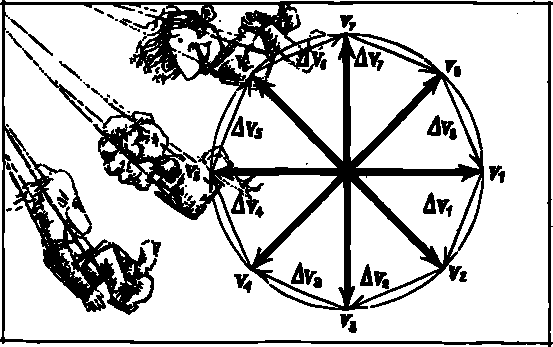
\includegraphics[width=\textwidth]{figures/fig-02-05.pdf}
\caption{Changes in velocity during a revolution of a body.}
\label{fig-2.05}
\end{figure}
The sum of the magnitudes of the changes in velocity
during a complete revolution will be equal to the sum
of the sides of the depicted polygon. In constructing each
small triangle, we have implicitly assumed that the
velocity vector changed by jumps, but its direction is
actually changing continuously. It is perfectly clear that
the smaller we take the vertex angles of the small triangles, the less will be our error. The smaller the sides of our polygon, the closer will they cling to the circle of radius $v$. Consequently, the exact value of the sum of the magnitudes of the changes in velocity during the course of the revolution of a point will be the circumference
$2\pi v$ of the circle. The magnitude of the acceleration is found by dividing it by the time of a complete revolution $T$: 
\begin{equation*}
a = \frac{2\pi v}{T}
\end{equation*}
\begin{figure}[!ht]
\centering
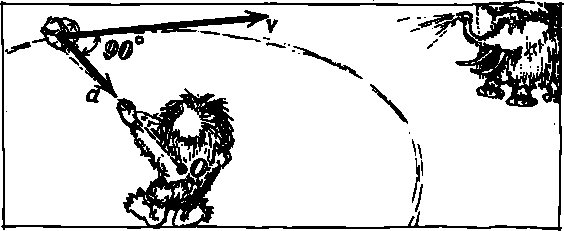
\includegraphics[width=\textwidth]{figures/fig-02-06.pdf}
\caption{Relationship between acceleration and velocity in circular motion.}
\label{fig-2.06}
\end{figure}
The time of a complete revolution in motion around
a circle of radius $R$ can be expressed in the form $T
= 2 \pi R/v$. Substituting this expression in the preceding
formula, we obtain the following for the acceleration:
$a = v^{2}/R$.

For a constant radius of rotation, the acceleration is
proportional to the square of the speed. For a given speed,
the acceleration is inversely proportional to the radius.
This same reasoning shows us how the acceleration of
a circular motion is directed at each given instant. The
smaller the vertex angle of the isosceles triangles which
we used for our proof, the nearer the angle between the
increment in velocity and the velocity will be to \ang{90}.

Therefore, the acceleration of a uniform circular motion
is directed perpendicular to the velocity; and how are the
velocity and acceleration directed relative to the trajectory? Since the velocity is tangent to the path, the acceleration is directed along the radius towards the centre of the circle. These relationships are clearly seen in \figr{fig-2.06}.

Try to twirl a stone on a string. You will clearly feel
the need for muscular exertion in order to do this. And
why is force necessary? After all, isn't the body moving
uniformly? The whole point here is that it isn't! The body
is moving with a constant speed, but the continuous change
in the direction of the velocity makes this motion accelerated. Force is necessary in order to deflect the body from an inertial straight path. Force is needed in order to create the acceleration $v^{2}/R$, which we have just computed.

According to Newton's law, force in always pointed
in the direction of the corresponding acceleration. Consequently, a body revolving around a circle with a constant speed should be subject to the action of a force directed along a radius towards the centre of the circle. The force acting on the stone exerted by the string is
called \emph{centripetal}; it is just this force that supplies the
acceleration $v^{2}/R$. Hence, the magnitude of this force
is $m v^{2}/R$.\label{cp}

The string pulls the stone; the stone pulls the string.
In these two forces we recognize ``an object and its mirror
image'' -- forces of action and reaction. The force with
which the stone acts on the string is frequently called
centrifugal. The centrifugal force is, of course, equal to
$m v^{2}/R$ and directed along the radius out from the centre
of the circle. The centrifugal force acts on the body counteracting the tendency of the revolving body to move rectilinearly.

What we have said applies also to the case when the
role of the string is played by gravity. The Moon revolves
around the Earth. What is it that retains our satellite?
Why doesn't it go off, following the law of inertia, in
an interplanetary trip? The Earth is holding on to the
Moon with an ``invisible string'' -- a \emph{gravitational} force.
This force is equal to $m v^{2}/R$, where $v$ is the speed of the
motion along the lunar orbit, and $R$ is the distance to the
Moon. The centrifugal force in this case acts on the Earth,
but, because of the Earth's great mass, it only slightly
influences the character of our planet's motion.

Suppose that it is required to send an artificial Earth
satellite into a circular orbit at a distance of \SI{300}{\kilo\meter} from the Earth's surface. What should be the speed of such a
satellite? At a distance of \SI{300}{\kilo\meter}, the acceleration of
free fall is somewhat less than on the surface of the Earth,
and is equal to \SI{8.9}{\meter\per\second\squared}. The acceleration of a satellite moving in a circle is equal to $v^{2}/R$, where $R$ is the distance from the centre of the circle (i.e. from the centre of the
Earth) -- about $\SI{6600}{\kilo\meter} = \SI{6.6d6}{\meter}$. On the other hand, this acceleration is equal to the acceleration of free
fall, $g$. Consequently, $g = v^{2}/R$, from which we find
the speed of the satellite's orbital motion:
\begin{align*}
v & = \sqrt{gR} = \sqrt{8.9 \times \num{6.6d6}} \\
& = \SI{7700}{\meter\per\second} = \SI{7.7}{\kilo\meter\per\second}
\end{align*}
The minimum speed necessary for a body thrown horizontally to become an Earth satellite is called the orbital velocity. It is clear from the example we have given that this speed is close to \SI{8}{\kilo\meter\per\second}.


\section{Life at \emph{g} Zero}

Above we found a ``reasonable point of view'' on motion.
True, the ``reasonable'' points of view, which we called
inertial frames of reference, turned out to be infinite in
number.

Now, armed with a knowledge of the laws of motion,
we can become interested in what motion looks like
from an ``unreasonable'' point of view. Our interest in
how inhabitants of non-inertial frames of reference live
is by no means idle, if only because we ourselves are
dwelling in such a system.

Let us imagine that having grabbed our measuring
instruments we settled down in an interplanetary space-ship and went travelling in the starry world.

Time flies quickly. The Sun already resembles a little
star. The engine has been cut off and the ship is far away
from gravitating bodies.

Let us now see what's going on in our flying laboratory.
Why does the thermometer that slid off its nail float in
the air and not fall to the floor? In what a strange position
deviating from the ``vertical'' has the pendulum hanging
on the wall got stuck! We immediately find the solution:
after all, the ship is not on the Earth but in interplanetary
space. The objects have lost their weight.

Having feasted our eyes on this extraordinary scene,
we decide to change our course. We turn on the jet engine
by pressing a button, and suddenly \ldots{} the objects surrounding us seemed to come to life. All bodies which
hadn't been made fast were brought into motion. The
thermometer fell down, the pendulum began oscillating
and gradually coming to rest assumed a vertical position,
the pillow obediently sagged under the weight of the
valise lying on it. Let us take a look at the instruments
which indicate the direction in which our ship started
accelerating. Upwards, of course! The instruments show
that we chose a motion with an acceleration of \SI{9.8}{\meter\per\second\squared}, not very great considering the possibilities of our ship. Our sensations are quite ordinary; we feel the way we did on Earth. But why so? As before, we are unimaginably
far from gravitational masses, there is no gravity but
objects have acquired weight.

Let us drop a marble and measure the acceleration with which it falls to the floor of the spaceship. It turns out that the acceleration is equal to \SI{9.8}{\meter\per\second\squared}. This is the number we have just read on the instruments measuring the acceleration of the rocket. The ship is moving upwards with the same acceleration with which the bodies in our flying laboratory are falling downwards.
But what is ``up'' or ``down'' in a flying ship? How simple
things were when we lived on the Earth. There the sky
was up and the Earth was down. And here? Our up has
one unquestionable property -- it is the direction of the
acceleration of the rocket.

It isn't difficult to understand the meaning of our
observations: no forces were acting on the marble we
dropped. It moves by inertia, whereas the rocket moves
with an acceleration relative to the marble. To us who
are inside the rocket it seems that the marble is falling
in the direction opposite to that of the acceleration of the
rocket. Naturally, the acceleration of this fall is equal
in magnitude to the true acceleration of the rocket. It
is also clear that all bodies in the rocket will ``fall'' with
the same acceleration.

We may draw an interesting conclusion from all that
has been said. Bodies start ``weighing'' when the rocket
accelerates. Moreover, the ``gravitational force'' has a
direction opposite to that of the acceleration of the rocket,
and the acceleration of free ``fall'' is equal in magnitude
to that of the motion of the jet ship. And what is most
remarkable is the fact that in practice we are unable to
distinguish the accelerated motion of a frame of reference
from the corresponding gravitational force.\footnote{Only in practice. There is a difference in principle. Gravitational forces on the Earth are directed along radii towards the Earth's centre. This means that the directions of acceleration at two different points form an angle. In a rocket moving with an acceleration, the directions of weight are strictly parallel at all points. Acceleration also changes with height on the Earth; this effect is absent in an accelerating rocket.} If we were inside a spaceship with closed windows, we could not tell
whether we were at rest on the Earth or moving with
an acceleration of \SI{9.8}{\meter\per\second\squared} This indistinguishability of an acceleration from the action of a gravitational force is called in physics the \emph{equivalence principle}\label{eqpr}.

\begin{figure}[!ht]
\centering
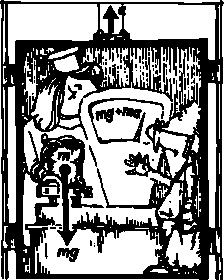
\includegraphics[width=\textwidth]{figures/fig-02-07.pdf}
\caption{The equivalence principle.}
\label{fig-2.07}
\end{figure}

This principle, as we shall now see illustrated by a
series of examples, permits one to quickly solve many
problems by adding to real forces the fictitious gravitational force existing in an accelerating frame of reference.

The elevator can serve as our first example. Let us take
along a spring balance with weights and go up in an
elevator. We shall follow the behaviour of the pointer
of the scale after placing a kilogram of vegetables on it
(\figr{fig-2.07}). The ascent has begun; we see that the scale
reading has increased, as though the weight weighed more
than a kilogram. The equivalence principle will easily
explain this fact. During the upward motion of the
elevator with an acceleration $a$, there arises an additional
gravitational force directed downwards. Since the acceleration of this force is equal to $a$, the additional weight is equal to $ma$. Hence, the scale shows a weight of $mg + ma$. The acceleration has ended, and the elevator is moving uniformly -- the scale has returned to its initial position and shows a weight of \SI{1}{\kilo\gram}. We are getting close to the top. floor, and the motion of the elevator is slowing down. What will now happen to the spring balance?

Well, of course, the load now weighs less than one kilogram. When the motion is slowing down, the acceleration vector points downwards. Therefore, an additional fictitious gravitational force is directed upwards, opposite to the direction of the Earth's gravitation. Now a is
negative, and so the scale shows a quantity less than $mg$. After the elevator comes to a halt, the scale returns to its initial position. 

Let us begin the descent. The motion of the elevator speeds up; the acceleration vector is directed downwards; hence, an additional gravitational force is directed upwards. The load now weighs less than
a kilogram. When the motion becomes uniform, the additional weight disappears, and towards the end of our trip on the elevator -- when the downward motion is decelerating -- the load will weigh more than a kilogram.

The unpleasant sensations experienced in rapidly accelerating and decelerating elevators are related to the change in weight under consideration.

If an elevator is falling with an acceleration, the bodies
inside it seem to become lighter. The greater this acceleration, the greater will be the loss of weight. But what will happen when a frame of reference falls freely? The answer is clear: in this case, bodies stop pressing down on the scale -- cease weighing: the Earth's gravitation will be balanced by the additional gravitational force existing in such a freely falling frame of reference. Being in such an ``elevator'', one can calmly place a ton on one's shoulders.

At the beginning of this section, we described life at
$g$ zero in an interplanetary spaceship which has left the
sphere of gravitation. There is no weight in such a spaceship during uniform rectilinear motion, but the same thing also takes place during the free fall of a frame of reference. Hence, there is no need to leave the sphere of gravitation. Weight is. absent in every interplanetary
ship which is moving with its engine cut off. A free
fall leads to the loss of weight in such systems. The equivalence principle brought us to the conclusion that a
frame of reference moving rectilinearly and uniformly
far from the action of gravitational forces is almost (see
the footnote on p.~\pageref{eqpr}) completely equivalent to a frame
of reference falling freely under the action of its weight.
In the first system there is no weight, and in the second
the ``downward weight'' is balanced out by the ``upward weight'' We will not detect any difference between these systems.

Life at $g$ zero begins in an artificial Earth satellite at the moment when the ship is orbited and begins moving without the aid of a rocket.

The first space traveller was the dog Laika, and soon afterwards a human being adapted to life at $g$ zero in the cabin of the spaceship. The Soviet cosmonaut, Yuri Gagarin, was the first to do so.

Life in the cabin of a spaceship cannot be called ordinary. A great deal of inventiveness and ingenuity were
needed in order to make objects so easily subordinated
by gravity obedient. Is it possible, for example, to pour
water from a bottle into a glass? For water pours ``downwards'' under the action of gravity. Is it possible to cook
food if water cannot be heated on a stove? (Warm water
will not mix with cold one.) How can one write with
a pencil on paper if a slight push of the former against
a table is enough to drive him aside? Neither a match
nor a candle nor a gas burner will burn, since burned-up
gases will not rise upwards (after all, there is no up!) to
make room for oxygen. It was even necessary to think
about how to guarantee a normal course for the natural
processes occurring in the human organism, for these
processes are ``accustomed'' to the Earth's gravitation.


\section{Motion from an ``Unreasonable'' Point of View}

Let us now take up the question of physical observations in an accelerating bus or streetcar. A peculiarity of
this example distinguishing it from the preceding one
consists in the following. In the example with the elevator, the additional weight and the Earth's gravitation
were directed along a single line. In a decelerating or
accelerating streetcar, the additional weight is directed
at right angles to the Earth's gravitation. This induces
distinctive, although customary, sensation in the passenger. If the streetcar increases its speed, there arises
an additional force opposite in direction to that of motion.

Let us add this force to that of the Earth's gravitation.
The resultant force acting on a person in the car will be
directed at an obtuse angle to the direction of the motion.
Standing, as usual, face forward in the car, we sense
that our ``upwards'' has moved. In order not to fall, we
shall want to become ``vertical'' -- as shown in \figr{fig-2.08}~\textcolor{black!70}{(a)}.
Our ``vertical'' is slanting. It is inclined at an acute angle
to the direction of the motion. If a person stands at
right angles to the motion without holding on to any-
thing, he will be sure to fall backwards.

\begin{figure}[!ht]
\centering
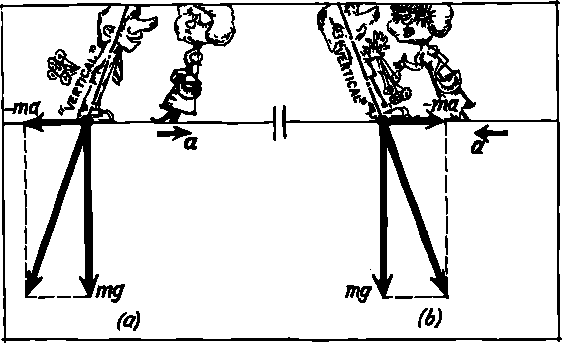
\includegraphics[width=\textwidth]{figures/fig-02-08.pdf}
\caption{The changing ``vertical''.}
\label{fig-2.08}
\end{figure}


Finally, the motion of the streetcar becomes uniform,
and we can stand calmly. However, we are drawing close
our to the next stop. The driver applies the brakes and
``vertical'' is deviating. It is now directed, as can be seen
from the drawing in \figr{fig-2.08}~\textcolor{black!70}{(b)}, at an obtuse angle to
the motion. In order not to fall, the passenger leans
backwards. However, he won't remain long in such
a position. The car comes to a halt, the deceleration
disappears, and the ``vertical'' is now directed at right
angles to the Earth. The position of one's body must
again be changed. Check your sensations. Isn't it true
that when the deceleration began you seemed to be pushed from behind, and when the car came to a halt you seemed to be pushed in your chest.

Similar phenomena also occur when a streetcar moves
around a curve. We know that motion around a circle,
even with a constant speed, is accelerated. The faster the
streetcar moves and the smaller the radius of curvature $R$, the greater the acceleration $v^{2} /R$. The acceleration
of such a motion is directed along a radius towards the
centre. But this is equivalent to the appearance of an
additional force directed outwards from the centre.
Therefore, an additional force of $mv^{2}/R$ will be acting
on a streetcar passenger during a turn throwing him out
towards the external side of the curve. The radial force
$mv^{2}/R$ is called centrifugal. We have already met this
force before, on p.~\pageref{cp} (true, considered from a somewhat
different point of view).

The action of a centrifugal force during the turning of a streetcar or a bus can only lead to a slight unpleasantness. The force $mv^{2}/R$ is not large in this case. However, during a speedy motion around a curve, the centrifugal force can become great enough to pose a threat to one's
life. Pilots come across large values of $mv^{2}/R$ when their
airplanes ``loop-the-loop''. While the airplane is describing a circle, the centrifugal force acts on the pilot pinning him to his seat. The smaller the circumference of the loop, the greater the additional force with which the pilot is pinned to the seat. If this ``weight'' becomes
large enough, a person can be ``torn'' because tissues of living organism possess limited strength and cannot withstand an arbitrary weight.

But how much weight can a person ``put on'' without
seriously endangering his life? That depends on the
duration of the overload. If it lasts a fraction of a second,
a person is capable of withstanding an overload from
$7g$ to $9g$. During ten seconds a pilot can withstand an
overload from $3g$ to $5g$. Cosmonauts are interested in the
kind of overload a person is able to bear for tens of minutes
and even, perhaps, hours. In such cases, it is likely that
the overload should be considerably lighter.

Let us compute the radii of a loop which an airplane
flying at various speeds can describe without any danger
to the pilot. We shall use the acceleration $v^{2}/R = 4g$.
Then $R = v^{2}/4g$, and for a speed of $\SI{360}{\kilo\meter\per\hour} = \SI{100}{\meter\per\second}$ the radius of the loop is \SI{250}{\meter}. But if the speed is four times greater, i.e. \SI{1440}{\kilo\meter\per\hour} (and such speeds have already been surpassed by modern jet airplanes), the radius of the loop should be increased by a factor of 16. The minimum radius of the loop becomes equal to \SI{4}{\kilo\meter}.

\begin{figure}[!ht]
\centering
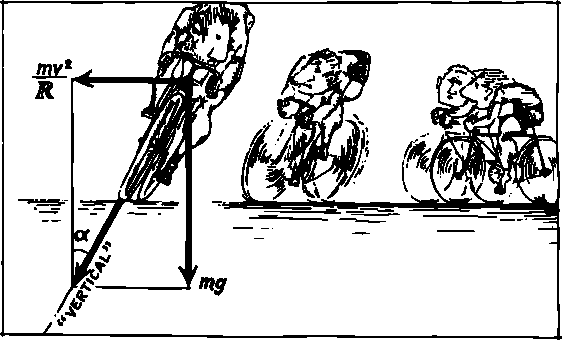
\includegraphics[width=\textwidth]{figures/fig-02-09.pdf}
\caption{To every rotational velocity there corresponds a distinct paraboloid.}
\label{fig-2.09}
\end{figure}

Nor shall we leave a more modest form of transportation -- the bicycle -- without attention. Everyone has seen
how a cyclist inclines while rounding a turn. Let us
suggest to a cyclist that he should ride around a circle
of radius $R$ with speed $v$, i.e. move with an acceleration $v^{2} / R$ directed towards the centre. Then besides the Earth's
gravitation an additional centrifugal force directed
horizontally outwards from the centre of the circle will
act on the cyclist. These forces and their sum are shown
in \figr{fig-2.09}. It is clear that the cyclist should hold himself ``vertically'', or else he will fall down. But \ldots{} his
vertical does not coincide with that of the Earth. It
can be seen from the figure that the vectors $mv^{2}/R$ and
$mg$ are the legs of a right triangle. 
\begin{figure}[!ht]
\centering
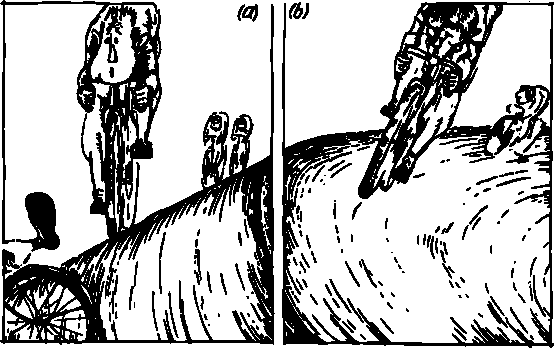
\includegraphics[width=\textwidth]{figures/fig-02-10.pdf}
\caption{To every rotational velocity, there corresponds a distinct paraboloid.}
\label{fig-2.10}
\end{figure}

The ratio of the leg opposite angle $\alpha$ to the adjacent one is called the tangent of angle $\alpha$ in trigonometry. We have $\tan \alpha = v^{2} /R g$; the mass has been cancelled out in full agreement with the equivalence principle. Hence, the cyclist's angle of
inclination does not depend on his mass-both a stout
and a thin riders must incline identically. The formula
and the triangle drawn in the figure show the dependence
of the incline on the speed of motion (it grows as the
latter increases) and the radius of the circle (it increases
as the latter decreases). We have explained why the
vertical of the cyclist does not coincide with that of
the Earth. What then will he feel? We must rotate
\figr{fig-2.09} in order to find it out. The road now looks
like the slope of a mountain (\figr{fig-2.10}~\textcolor{black!70}{(a)}), and it becomes clear to us that if the force of friction between the tires and the asphalt is insufficient (for example, when
the road is wet), the bicycle may slip and a sharp turn
may end with a fall into a ditch.

In order to forestall this, highways are built with
sharp turns inclined, i.e. horizontal for a cyclist -- as
shown in \figr{fig-2.10}~\textcolor{black!70}{(b)}. In this way, the tendency to slip can be greatly diminished, or even entirely eliminated. This is precisely how turns are constructed in bicycle
tracks and superhighways.

\section{Centrifugal Forces}
\label{centrifugal}
Let us now deal with rotating systems. The motion of
such a system is determined by the number of revolutions
per second which it makes about an axis. It is also necessary, of course, to know the direction of the axis of rotation.

In order to better understand the peculiarities of life
in rotating systems, let us consider the ``wheel of laughs'' --
a well-known ride. Its construction is rather simple.
A smooth disc, several metres in diameter, rotates rapidly.
Those who so desire are invited to get on it and to try
to keep their balance. Even people who know no physics
quickly acquire the secret of success: one must go to
the centre of the disc, since the farther one is from the
centre, the more difficult it is to keep one's balance.

Such a disc is a non-inertial frame of reference with
several special features. Every object attached to the
disc moves around a circle of radius $R$ with speed $v$,
i.e. with acceleration $v^{2}/R$. As we already know, from
the point of view of a non-inertial observer this implies
the presence of an additional force $mv^{2}/R$ directed along
the radius outwards from the centre. This radial force
will act at each point of the ``devilish wheel'' creating
there a radial acceleration $v^{2}/R$. The magnitude of this
acceleration will be identical for points lying on the same
circle. And what about points on different circles? Don't
rush to answer that according to the formula $v^{2}/R$ the
smaller the distance from the centre, the greater will be
the acceleration. This isn't true because the speed of
points farther from the centre of the wheel will be greater.
In fact, if the wheel makes $n$ revolutions per second,
the path traversed by a point on the rim of the wheel
in one second (the speed of this point) is $2\pi R n$.

The speed of a point is directly proportional to its
distance from the centre. We may now rewrite our formula for the acceleration:
\begin{equation*}
a = 4 \pi^{2} n^{2} R
\end{equation*}
Since the number of revolutions made in a second is the
same for all points of the wheel, we arrive at the following result: the acceleration due to the force exerted by
the ``radial gravity'' acting on a rotating wheel grows in
proportion to the distance of a point from the centre
of the wheel.

In this interesting non-inertial frame of reference the
force of gravity is different on different circles. Therefore,
the directions of the ``verticals'' will also be different for
bodies located at different distances from the centre.
The Earth's gravitational force is, of course, the same
at all points of the wheel. But the vector characterizing
the additional radial force becomes longer as the distance
from the centre increases. Therefore, the diagonals of
the rectangles deviate more and more from the vertical
(normal to the Earth's surface).

If we imagine the successive sensations of a person
slipping off the ``wheel of laughs'', from his point of view
it can be said that the farther one gets from the centre,
the more the disc ``inclines'' making it impossible to stay
on it. To keep his place on the turntable, he must try
to place his centre of gravity on a ``vertical'' inclined in
such a way that the farther he is from the rotation axis,
the greater the inclination angle (\figr{fig-2.11}).

\begin{figure}[!ht]
\centering
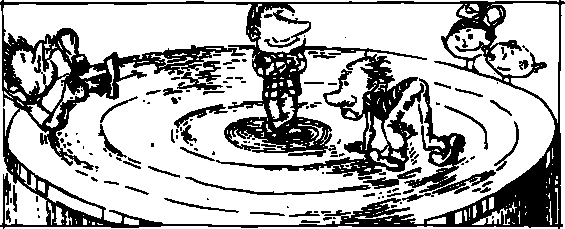
\includegraphics[width=\textwidth]{figures/fig-02-11.pdf}
\caption{A wheel of laughs. Farther a person is from the centre, more difficult it is to stay put.}
\label{fig-2.11}
\end{figure}

However, could it be possible to invent a contraption
analogous to an inclined highway for this inertial frame
of reference? Of course it is, but the disc would have to
be replaced by such a surface that the resultant gravitational force is perpendicular to it at each of its points.
The form of such a surface can be computed. It is called
a paraboloid. This name isn't accidental: every vertical
cut of a paraboloid is a parabola-the curve along which
bodies fall. A paraboloid is obtained by rotating a parabola around its axis.

It is very easy to create such a surface by making a vessel containing water rotate rapidly. The surface of the
rotating liquid is precisely a paraboloid. The water
particles will stop moving just when the force pressing
each particle to the surface is perpendicular to it. To
every rotational velocity there corresponds a distinct
paraboloid (\figr{fig-2.12}).

\begin{figure}[!ht]
\centering
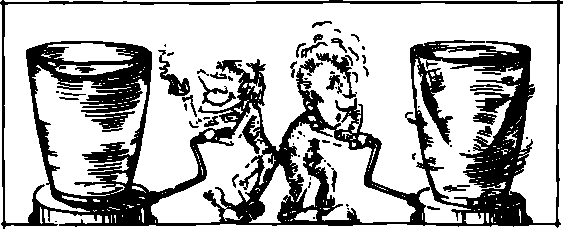
\includegraphics[width=\textwidth]{figures/fig-02-12.pdf}
\caption{To every rotational velocity there corresponds a distinct paraboloid.}
\label{fig-2.12}
\end{figure}


It is possible to demonstrate this property by making
a solid paraboloid. A small ball placed at any point
of a paraboloid rotating with a definite velocity will
remain at rest. This means that the force acting on it
will be perpendicular to the surface. In other words, a
rotating paraboloid behaves as a flat surface. One can
walk along such a surface and feel stable, just as on the
Earth. However, the direction of the vertical will change
during the walk.


Centrifugal phenomena are widely employed in technology. For example, the construction of a centrifuge is based on the use of these phenomena.


A centrifuge is a drum which rotates rapidly around its
axis. What will happen if various objects are thrown into
such a drum filled to the brim with water?

Let us drop a metal ball into the water -- it will go to
the bottom but not along our vertical; in moving away
from the axis of rotation all the time it will come to
a halt at the side. Now let us throw a cork ball into the
drum -- it, on the contrary, will immediately begin
moving towards the axis of rotation and settle there.

If the drum of this model of a centrifuge has a large
diameter, we shall notice that the acceleration increases
sharply as the ball moves away from the centre.

The phenomena which take place do not puzzle us at
all. There is an additional radial force within the centrifuge. If the centrifuge is rotating rapidly enough, its
``bottom'' is the lateral surface of the drum. The metal
ball ``sinks'' in the water, but the cork ball ``floats'' The
farther a body ``falling'' in the water is from the axis of
rotation, the ``heavier'' it becomes.

In sufficiently perfected centrifuges, the rotational
velocity can be raised to \num{60000} rpm, i.e. $10^{3}$ rps. At
a distance of \SI{10}{\centi\meter} from the axis of rotation, the acceleration due to the radial gravitational force will be approximately equal to
\begin{equation*}
40 \times 10^{6} \times 0.1 = 4 \times \SI{d6}{\meter\per\second\squared}
\end{equation*}
i.e. \num{400000} times greater than terrestrial acceleration.

It is clear that the Earth's gravitation may be neglected for such machines; we really have the right to regard the lateral surface of the drum as the ``bottom'' in a centrifuge.

The fields of application of a centrifuge become clear
from what we have said. If we want to separate the heavy
particles in a mixture from the light ones, it is always
advisable to apply a centrifuge. Everybody knows the
expression: ``The muddy liquid has settled.'' If dirty
water stands long enough, the sediment (usually heavier
than the water) will settle to the bottom. However, the
process of settling may take months, but with the aid
of a good centrifuge it is possible to clean up the water
instantly.

Centrifuges rotating with velocities of tens of thousands
of revolutions per minute are capable of separating the
finest particles of sediment not only from water but also
from viscous fluids.

Centrifuges are applied in the chemical industry for
separating crystals from the solution out of which they
grew, for dehydrating salts and for cleaning varnishes;
they are used in the food industry for separating syrup
from sugar.

The centrifuges which are applied in separating solid
or liquid components from a large number of fluids are
called separators. Their main application is the processing
of milk. Milk separators whirl with velocities of 2000-6000 rpm; the diameters of their drums are as large
as \SI{5}{\meter}.

Centrifugal casting is widely applied in metallurgy.
Even at velocities of 300-500 rpm the liquid metal flowing
into the rotating cast is pressed against its outer surface
with a considerable force. Metal pipes cast by this method
are denser, more uniform and without blisters or cracks.

\begin{figure}[!ht]
\centering
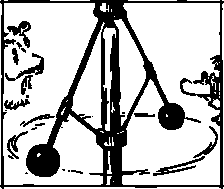
\includegraphics[width=0.6\textwidth]{figures/fig-02-13.pdf}
\caption{A centrifugal governor.}
\label{fig-2.13}
\end{figure}

Here is another application of centrifugal force. A
simple instrument that serves as a governor of the number
of revolutions of the rotating parts of a machine is depicted in \figr{fig-2.13}. This instrument is called a centrifugal governor. As the velocity of rotation increases, the centrifugal force grows, and the small balls of the governor move farther away from its axis. The rods attached to the balls are deflected, and when the deflection
reaches a definite level computed by an engineer, some electrical contacts may be broken, and in the case of a steam engine, for example, valves may be opened letting out excess steam. This will decrease the velocity of rotation and return the rods to their normal position.

Here is an interesting experiment. Place a small cardboard disc on the axis of an electric motor. Switch on the electricity and bring a piece of wood in contact with the whirling disc. A fairly thick beam can be sawed in half as easily as by a steel saw.

An attempt to saw wood by means of cardboard can
only evince a smile if one employs it as a hand saw.
Why then does the rotating cardboard cut wood? The
cardboard particles on the boundary of the disc experience
an enormous centrifugal force. The lateral forces which might alter the plane of the cardboard are insignificant in comparison with the centrifugal ones. By keeping its plane fixed, the cardboard disc acquires the ability of gnawing
into the wood.

The centrifugal force arising as a result of the Earth's
rotation leads to the differences in the weight of a body
at various latitudes that we spoke of above.

A body weighs less at the equator than at a pole for
two reasons. Bodies lying on the Earth's surface are at
different distances from the Earth's axis depending on
the latitude of their locations. Of course, this distance
grows in passing from a pole to the equator. Moreover, a
body located at a pole is on the axis of rotation, so the
centrifugal acceleration is 
\begin{equation*}%
a = 4 \pi^{2}n^{2}R = 0
\end{equation*}
(the distance from the axis of rotation $R = 0$). At the equator, on the contrary, this acceleration is maximum.

The centrifugal force reduces the gravitational force. Therefore, the pressure exerted by a body on a scale (the weight of the body) is minimum at the equator.

If the Earth had a precisely spherical form, then a kilogram weight carried from a pole to the equator would lose \SI{3.5}{\gram} in weight. You can easily find this number if you use the expression $4\pi^{2}n^{2}Rm$ and substitute $n = 1$ revolution per day, $R = \SI{6300}{\kilo\meter}$, and $m = \SI{1000}{\gram}$. Only don't forget to convert the units of measurements to seconds and centimetres.

However, a kilogram weight will actually lose \SI{5.3}{\gram},
and not \SI{3.5}{\gram}. This is the case because the Earth is an
oblate sphere called an ellipsoid in geometry. The distance
from a pole to the centre of the Earth is about 1/300 less
than a terrestrial radius extended to the equator. 

This contraction of the Earth was caused by the very same centrifugal force. In fact, it is exerted on all the particles of the Earth. In remote times, the centrifugal force ``moulded'' our planet-gave it an oblate form.

\section{Coriolis Forces}
The peculiarities of the world of rotating systems are
not exhausted by the existence of radial gravitational
forces. We shall become acquainted with still another
interesting effect whose theory was presented in 1835
by the Frenchman Gaspard Gustave de Coriolis (1792-1843).

Let us pose the following question: What does rectilinear motion look like from the point of view of a rotating laboratory? A design of such a laboratory is depicted
in \figr{fig-2.14}. The rectilinear trajectory of some body is
shown by means of a ray passing through the centre. We
are considering the case when the path of the body passes
through the centre of rotation of our laboratory. The
disc on which the laboratory is standing rotates uniformly; five positions of the laboratory with respect to the
rectilinear trajectory are shown in the figure. This is
how the relative positions of the laboratory and the
trajectory of the body look after one, two, three, etc.,
seconds. The laboratory, as you see, is rotating counter-clockwise if looked upon from above.

\begin{figure}[!ht]
\centering
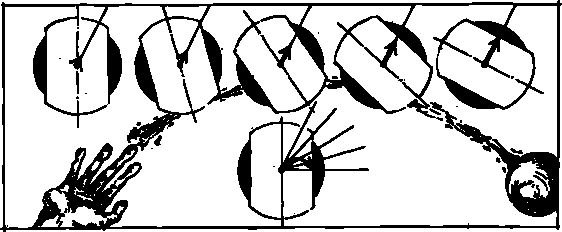
\includegraphics[width=\textwidth]{figures/fig-02-14.pdf}
\caption{A view from a rotating laboratory.}
\label{fig-2.14}
\end{figure}

Arrows corresponding to the segments through which
the body passes during one, two, three, etc., seconds have
been drawn on the line of its path. The body covers the
same distance during each second, since we are dealing
with uniform and rectilinear motion from the point
of view of a fixed observer.


Imagine that the moving body is a freshly painted ball
rolling along the disc. What kind of trace will remain on
the disc? Our construction yields the answer to this
question. The points which mark the ends of the arrows
have been transferred from our five drawings to a single
diagram. It remains to connect these points by a smooth
curve. The result of our construction will not surprise
us: rectilinear and uniform motion looks like curvilinear
motion from the point of view of a rotating observer. The
following rule attracts our attention: a moving body is
deflected to the right of its path during the entire course
of the motion. We now assume that the disc is rotating in
the clockwise direction, and leave the repetition of our
construction to the reader. It will show that, in this
case, a moving body is deflected to the left of its path
from the point of view of a rotating observer.

We know that a centrifugal force arises in rotating
systems. However, its action cannot serve as the cause of
the deformation of the path, for it is directed along the
radius. Hence, besides the centrifugal force another
additional force arises in rotating systems. It is called
the \emph{Coriolis force}.

Why is it that in the previous examples we did not
come across the Coriolis force and managed superbly with
only centrifugal? The reason is that until now we have
not regarded motion from the point of view of a rotating observer, and a Coriolis force arises only in such a case.
Only a centrifugal force is exerted on bodies which are,
stationary in rotating systems. A table in a rotating
laboratory is screwed on to the floor -- only a centrifugal
force is exerted on it. But on a ball which has fallen
from the table and rolled along the floor of the rotating
laboratory besides a centrifugal force a Coriolis force
is also exerted.

On what quantities does the magnitude of a Coriolis
force depend? It can be calculated, but the computations
are too complicated to be given here. We shall therefore
present only the result of these computations.

Unlike a centrifugal force whose magnitude depends
on the distance from the axis of rotation, a Coriolis force
is independent of the position of a body. It is determined
by the velocity vector (i.e. not only by its magnitude,
but also by its direction with respect to the axis of rotation). If the body moves along the axis of rotation, the
Coriolis force is equal to zero. The greater the angle
between the velocity vector and the axis of rotation, the
greater will be the Coriolis force; this force assumes its
maximum value when the motion of the body is at right
angles to the axis. As we know, it is always possible to
decompose a velocity vector into any pair of its components and consider separately the two resulting motions
in which the body is simultaneously involved.

If the velocity of a body is decomposed into components $v_{\parallel}$ and $v_{\perp}$ -- parallel and perpendicular to the axis of rotation -- then the first motion will not be subject
to the action of a Coriolis force. The magnitude of the
Coriolis force $F_{C}$ is determined by the component $v_{\perp}$
of the velocity. Computations lead to the formula
\begin{equation*}%
F_{C}= 4 \pi n v_{\perp} m
\end{equation*}
Here $m$ is the mass of the body, and $n$ is the number of
revolutions made by the rotating system in a unit of time. As can be seen from the formula, the faster the system rotates and the faster the body moves, the greater will be the Coriolis force.

Calculations also established the direction of a Coriolis force. This force is always perpendicular to the axis of rotation and the direction of the motion. Moreover, as has already been said above, the force is directed to the right of its path in a system rotating counterclockwise.

Many interesting phenomena occurring on the Earth
are explained by the action of Coriolis forces. The Earth
is a sphere, and not a disc. This makes the effect of
Coriolis forces more complicated. These forces will not
only influence motion along the Earth's surface but also
the falling of bodies to the Earth.

Does a body fall exactly along a vertical? Not quite.
Only at a pole does a body fall exactly along a vertical.
Here the direction of the motion and the Earth's axis of
rotation coincide, so there is no Coriolis force. The situation is different at the equator; here the direction of
the motion forms right angles with the Earth's axis.
If looked upon from the North Pole, the Earth's rotation
will appear to be counterclockwise. Hence, a freely falling
body should be deflected to the right of its path, i.e.
to the East. The magnitude of this eastward deflection,
the greatest at the equator, decreases to zero as the poles
are approached.

Let us compute the magnitude of the deflection at the
equator. Since a freely falling body moves with a uniform
acceleration, the Coriolis force increases as the Earth
is approached. We shall therefore restrict ourselves to
an approximate computation. If the body falls from a
height, say, of \SI{80}{\meter}, its fall will last about \SI{4}{\second} according to the formula $t = \sqrt{2h/g}$. The average speed for the fall will be equal to \SI{20}{\meter\per\second}.

This is the speed that we shall substitute in our formula
for the Coriolis acceleration, $4 \pi n v$ Let us convert the
value $n = 1$ revolution in 24 hours to the number of
revolutions per second; $24 \times 3600$ seconds are contained
in 24 hours, so $n$ is equal to 1/86,400 rps: consequently,
the acceleration created by the Coriolis force is equal to
$\pi/\SI{1080}{\meter\per\second\squared}$ The distance covered during \SI{4}{\second} with such an acceleration is equal to $(1/2) (\pi/1080) \times 4^{2} = \SI{2.3}{\centi\meter}$. This is precisely the magnitude of the eastward deflection in our example. An exact computation, taking into
account the non-uniformity of the fall, yields a close but
somewhat different number.

While the deflection of a freely falling body is maximum at the equator and equal to zero at the poles, we shall see the opposite picture in the case of the deflection of a body moving in a horizontal plane under the action of a Coriolis force.

A horizontal site on the North or South Pole does not
differ at all from the rotating disc with which we began
our study of Coriolis forces. A body moving along such a
site will be deflected to the right of its path by the Coriolis
force at the North Pole, and to the left at the South Pole.
Using the same formula for the Coriolis acceleration, the
reader can calculate without difficulty that a bullet fired
from a rifle with an initial speed of \SI{500}{\meter\per\second} will be deflected from the target by \SI{3.5}{\centi\meter} in a horizontal plane during one second (i.e. while it travels \SI{500}{\meter}).
\begin{figure}[!ht]
\centering
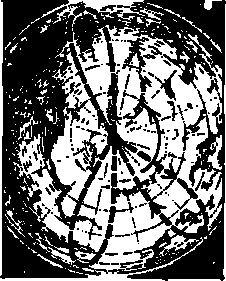
\includegraphics[width=0.7\textwidth]{figures/fig-02-15.pdf}
\caption{The Foucault's pendulum.}
\label{fig-2.15}
\end{figure}

But why should the deflection in a horizontal plane at
the equator be equal to zero? Without rigorous proofs,
it is clear that this should be the case. At the North
Pole a body is deflected to the right of its path, and at
the South Pole to the left, hence, half-way between the
poles, i.e. at the equator, the deflection will be equal to zero. Let us recall the experiment with the Foucault pendulum. A pendulum oscillating at a pole preserves the plane
of its oscillations. The Earth in its rotation moves away
from under the pendulum. This is how the stellar observer
explains the Foucault experiment. But the observer rotating together with the Earth explains this experiment
by means of a Coriolis force. As a matter of fact, a Coriolis
force is directed perpendicularly to the Earth's axis
and perpendicularly to the direction of the motion of the
pendulum; in other words, the force is perpendicular
to the plane of the oscillation of the pendulum and will
continually turn this plane. It can be arranged so that
the end of the pendulum traces the trajectory of the
motion. This trajectory is represented by the ``rosette''
shown in \figr{fig-2.15}. It can be seen from this figure
that the ``Earth'' completes one quarter of a rotation
during one and a half periods of the oscillation of the
pendulum. The Foucault pendulum turns much more
slowly. At a pole, the plane of oscillation of the pendulum
will turn through one-fourth of a degree during one
minute. At the North Pole the plane will be turned to
the right of the path of the pendulum, and at the South
Pole to the left.

\begin{figure}[!ht]
\centering
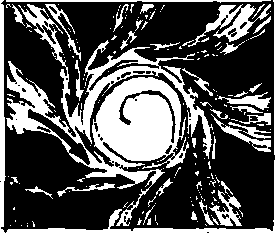
\includegraphics[width=0.7\textwidth]{figures/fig-02-16.pdf}
\caption{The Coriolis effect and cyclones.}
\label{fig-2.16}
\end{figure}

The Coriolis effect will be somewhat less at Central European latitudes than at the equator. A bullet in the example we have just given will be deflected not by \SI{3.5}{\centi\meter} but by \SI{2.5}{\centi\meter}. The Foucault pendulum will be turned by about one-sixth of a degree during one minute.

Must a gunner take the Coriolis force into account?
Big Bertha used by the Germans to shell Paris during
World War I was situated \SI{110}{\kilo\meter} from the target. The
Coriolis deflection is as much as \SI{1600}{\meter} in such a case.
This is no longer a small quantity. If a flying projectile
is sent very far without taking the Coriolis force into
account, it will be deflected significantly from its course.
This effect is large not because the force is great (for a ten
ton projectile having a speed of \SI{1000}{\kilo\meter\per\hour}, the Coriolis force will be about \SI{25}{\kgf}) but because it is exerted
continually for a long period of time.

Of course, the influence of wind on a rocket projectile
may be no less significant. Flight corrections made by
a pilot depend on the action of the wind, the Coriolis
effect and imperfections in the airplane or flying bomb.

What specialists besides aviators and gunners should
be aware of the Coriolis effect? Strange as it may seem,
among such specialists are railroaders. Under the action
of the Coriolis force, one of the rails of a railroad wears
out on the inside noticeably more than the other. We
know just which one: in the Northern Hemisphere it will
be the right rail (relative to the motion of a train), and
in the Southern Hemisphere the left one. Only the railroaders in equatorial countries are saved from trouble
in connection with this.

\begin{figure}[!ht]
\centering
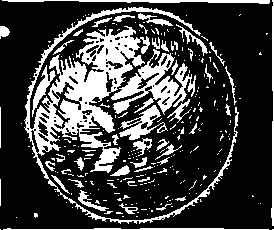
\includegraphics[width=0.7\textwidth]{figures/fig-02-17.pdf}
\caption{The trade winds.}
\label{fig-2.17}
\end{figure}


The washing away of right banks in the Northern
Hemisphere is explained in exactly the same way as the
wearing out of rails. The deviation of a river bed is to
a large extent related to the action of the Coriolis force.
It turns out that rivers in the Northern Hemisphere pass
obstacles on the right.

It is known that streams of air flow into a low-pressure
area. But why is such a wind called a cyclone? After all,
the root of this word suggests a circular (cyclic) motion.

This is precisely the case -- a circular motion of air
masses arises in a low-pressure area (\figr{fig-2.16}). The
cause lies in the action of the Coriolis force. In the Northern Hemisphere all air streams directed towards the low-pressure area are deflected to the right of their motion. Take a look at \figr{fig-2.17} -- you see that this leads to a westward deflection of the winds blowing in both hemispheres from the tropics to the equator (trade-winds). 

Why does such a small force play such a big role in the motion of air masses? This is explained by the insignificance of the frictional forces. Air is extremely mobile,
and a small but constantly acting force can lead to important consequences.
